\section{Graph Analysis with \method{}}
\label{sec:experiments}

\subsection{Data and Setup}
\label{sec:data}

\begin{table}[H]
\centering
\scriptsize
\setlength{\tabcolsep}{3pt}
\begin{tabularx}{\linewidth}{lrrX}
\toprule
\textbf{Split} & \textbf{Records} & \textbf{Models} & \textbf{Process focus} \\
\midrule
\mcp{} & 899 & 5 & MCP tool orchestration \\
\searchb{} & 3,270 & 5 & Web search and answer synthesis \\
\swe{} & 747 & 5 & Repository editing and tests \\
\taub{} & 984 & 5 & API use under policies \\
\terminal{} & 1,429 & 5 & Command-line tasks \\
\bottomrule
\end{tabularx}
\caption{Trajectory records in the five retained release splits before graph-validity filtering. Each task is attempted by five models with up to roughly four passes per model, with some missing or filtered attempts.}
\label{tab:data}
\end{table}

We analyze the gated cx-cmu agent trajectory release on Hugging Face~\citep{cxcmu2026agenttrajectories}.
The analyzed splits include tool orchestration, web-search answer synthesis, software repair, API-policy interaction, and command-line tasks from \mcp{}~\citep{wang2025mcpbench}, the \searchb{} split of the cx-cmu trajectory release~\citep{cxcmu2026agenttrajectories}, \swe{}~\citep{jimenez2024swebench}, \taub{}~\citep{barres2025tau2}, and \terminal{}~\citep{merrill2026terminalbench}.
The public dataset card describes several benchmark splits and multiple passes from the same five models on the same tasks; it records \searchb{} as a split label with web-search trajectories for answering complex questions, including \texttt{browsecomp}, \texttt{webvoyager}, and \texttt{mind2web} domains~\citep{cxcmu2026agenttrajectories}. We therefore use \searchb{} as the release split name rather than as a standalone benchmark title, while noting that the release tool inventory is reconstructed from the General-AgentBench source tree~\citep{cxcmu2026agenttrajectories,li2026generalagentbench}.
We use the five splits with rich tool or environment interaction and exclude the short math split, leaving a retained release subset of 7,329 trajectory records on 427 tasks before graph-validity filtering.
The analyzed trajectories are English-language task interactions with code, tool, or API observations.
The models are DeepSeek-R1, DeepSeek-V3.2, Gemini-2.5-Flash, Qwen3-235B, and Qwen3-Next.

For the four binary-reward splits, $y_r$ is the recorded binary success/reward flag: for example, \swe{} uses resolved-style issue success, whereas \searchb{} uses the binary \texttt{score} recorded in the release.
For \mcp{}, which reports a continuous multi-criteria score, we use per-task max-normalized reward.
This avoids introducing a binary threshold for a split that is near-saturated under a positive-reward rule.
For \searchb{}, we add pre-specified search-interaction keys for URL domain, query novelty, and cumulative source diversity; exact extraction rules are in Appendix~\ref{app:keys}.

\begin{figure*}[t]
\centering
\begin{subfigure}[t]{0.32\textwidth}
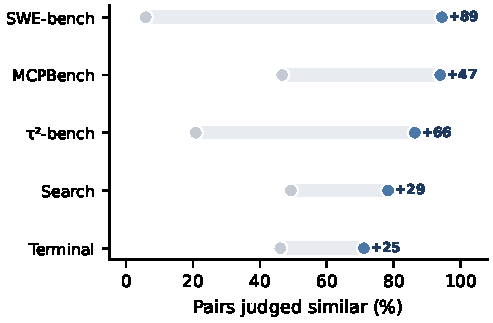
\includegraphics[width=\textwidth]{figures/fig3_panel_a.pdf}
\end{subfigure}\hfill
\begin{subfigure}[t]{0.32\textwidth}
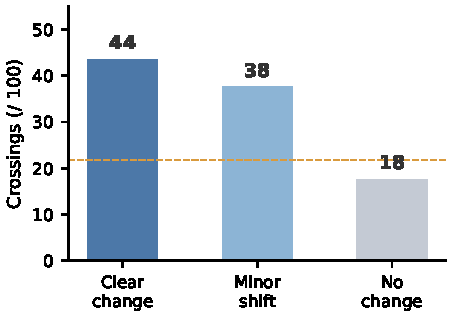
\includegraphics[width=\textwidth]{figures/fig3_panel_b.pdf}
\end{subfigure}\hfill
\begin{subfigure}[t]{0.32\textwidth}
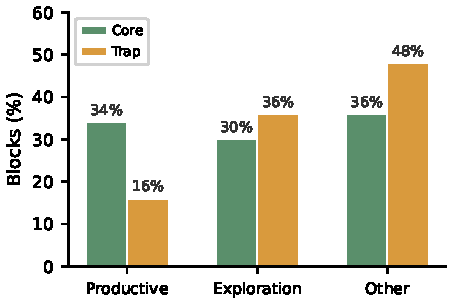
\includegraphics[width=\textwidth]{figures/fig3_panel_c.pdf}
\end{subfigure}
\caption{Human annotation checks for graph-derived states. \textbf{(a)}~Within-BCC step pairs are judged similar far more often than across-BCC pairs on every benchmark (overall $84.8\%$ vs. $40.2\%$ after dropping unsure labels; Fisher OR$\,{=}\,8.30$). \textbf{(b)}~Of 100 graph-identified articulation crossings, 82 show a strategy or phase change ($4.6\times$ the random baseline, dashed line). \textbf{(c)}~Core blocks are annotated as productive progress $2.1\times$ more often than trap blocks ($34\%$ vs. $16\%$); $36\%$ of trap blocks are exploration rather than dead ends.}
\label{fig:rq1_validity}
\end{figure*}

\subsection{Do \method{} Landscapes Expose Interpretable Agent States?}
\label{sec:rq1}

We first check whether a \method{} landscape is a usable measurement scaffold.
The evidence is deliberately modest: it asks whether the graph units are interpretable enough to support analysis, not whether every block has a perfect semantic label.

\paragraph{Block semantics.}
Two annotators scored 400 blinded BCC pairs, split evenly between within-BCC and across-BCC pairs.
After dropping unsure labels, within-BCC pairs were marked similar 84.8\% of the time (162/191), compared with 40.2\% for across-BCC pairs (72/179; Fisher exact OR=8.30, $p=1.4\times 10^{-19}$).
Per-benchmark gaps range from +89 percentage points on \swe{} to +25 percentage points on \terminal{}; \searchb{} has a +29 point gap under the pre-enrichment signature.
This supports reading BCCs as coarse shared agent states (Figure~\ref{fig:rq1_validity}a).

\paragraph{Articulations and regions.}
A second annotation pass scored 100 graph-identified articulation crossings.
Eighty-two show at least a minor strategy or phase change, a 4.6$\times$ enrichment over random consecutive steps (Figure~\ref{fig:rq1_validity}b).
We use this as a graph-construction sanity check, not as a main supply--demand axis.
A third pass scored 50 core blocks and 50 trap blocks.
Core blocks are 2.1$\times$ more likely than trap blocks to be judged productive progress (34\% vs. 16\%, Fisher $p=0.032$), and region-consistent extreme labels---productive core blocks and looping/dead-end trap blocks---outnumber inconsistent extremes 35 to 11.
However, 36\% of trap blocks are judged exploration, so a trap is best understood as a low-outcome region, not necessarily useless behavior (Figure~\ref{fig:rq1_validity}c).

\paragraph{Why a shared graph?}
Pooled graphs produce an average of 16.1 non-trivial blocks across 408 valid tasks, enough to compare several models as traffic on the same terrain.
Per-model graphs are much smaller because each model contributes only a few rollouts per task.
A representation ablation further shows that the full multi-channel signature has the broadest valid-task coverage; the ablation is kept in Appendix~\ref{app:signature_ablation} because it is a sanity check rather than the semantic core of the paper.

\subsection{What Process Profiles Do Models Exhibit?}
\label{sec:rq2}

Once the landscape is fixed, model identity is traffic over the same terrain.
Figure~\ref{fig:supply_demand}a shows model supply as a heatmap; exact values with bootstrap CIs are in Appendix Table~\ref{tab:model_profiles}.
Positive values mean the model exhibits that event more often than the average model on the same tasks; for Trap exposure, lower values mean more avoidance.

The profiles give model descriptions rather than a new ranking.
\textbf{DeepSeek-V3.2} is the clearest high-access, high-repair model: its Access and Repair CIs are both positive, while Trap is nearly neutral.
\textbf{Qwen3-Next} is low-access and low-repair, with lower Trap supply; this looks less like robust recovery and more like conservative, shallow navigation.
\textbf{Qwen3-235B} shows mildly elevated Access and marginally elevated Trap exposure, suggesting a less conservative exploration style, but its Repair interval overlaps zero.
\textbf{DeepSeek-R1} is near-balanced, and \textbf{Gemini-2.5-Flash} has lower Access and Repair supply in this corpus.

\begin{figure*}[t]
\centering
\begin{subfigure}[t]{0.48\textwidth}
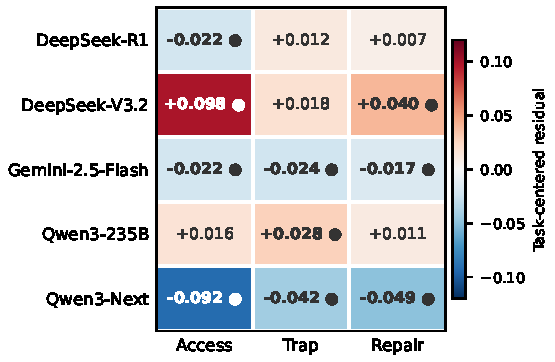
\includegraphics[width=\textwidth]{figures/fig4_panel_a.pdf}
\end{subfigure}\hfill
\begin{subfigure}[t]{0.48\textwidth}
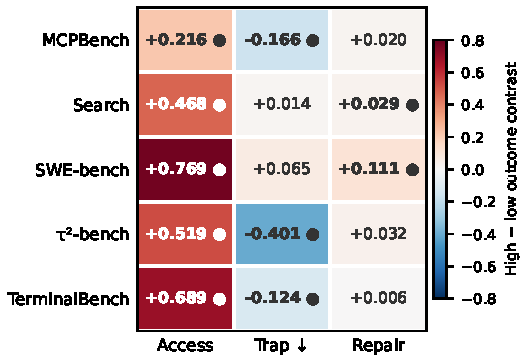
\includegraphics[width=\textwidth]{figures/fig4_panel_b.pdf}
\end{subfigure}
\caption{Supply--demand profile heatmaps. \textbf{(a)}~Model supply: task-centered event residuals; DeepSeek-V3.2 is distinctly high-Access/high-Repair, while Qwen3-Next is low on both. \textbf{(b)}~Benchmark demand: resolved-minus-failed contrasts (or the reward-weighted analogue on \mcp{}); Access is universally positive, \taub{} is strongly Trap-averse, \mcp{}/\terminal{} are also negative on Trap, and \swe{} has by far the strongest positive Repair demand. Filled markers~({\large$\bullet$}) denote 95\% bootstrap CIs excluding zero.}
\label{fig:supply_demand}
\end{figure*}

\begin{figure*}[t]
\centering
\begin{subfigure}[t]{0.32\textwidth}
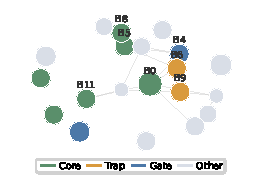
\includegraphics[width=\textwidth]{figures/fig5_panel_a.pdf}
\end{subfigure}\hfill
\begin{subfigure}[t]{0.32\textwidth}
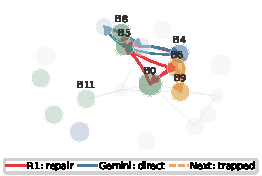
\includegraphics[width=\textwidth]{figures/fig5_panel_b.pdf}
\end{subfigure}\hfill
\begin{subfigure}[t]{0.32\textwidth}
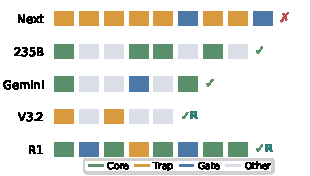
\includegraphics[width=\textwidth]{figures/fig5_panel_c.pdf}
\end{subfigure}
\caption{A shared landscape on \swe{} task \texttt{django-9296}. \textbf{(a)}~Block quotient graph: nodes are BCC blocks ({\color[HTML]{5A8F6B}green}=core, {\color[HTML]{D99A3D}amber}=trap, blue=articulation landmark, gray=other). \textbf{(b)}~Three trajectories as arrows: {\color[HTML]{E63946}DeepSeek-R1} repairs from B6 back to core; {\color[HTML]{457B9D}Gemini} navigates directly; {\color[HTML]{F4A261}Qwen3-Next} (dashed) cycles in B9$\leftrightarrow$B6 without escaping. \textbf{(c)}~Block ribbons per model; \checkmark/\texttimes\ marks resolution, \textbf{R} marks Repair.}
\label{fig:case_study}
\end{figure*}

\subsection{What Process Demands Do Benchmarks Impose?}
\label{sec:rq3}

We next ask which events separate high-outcome from low-outcome traffic inside each benchmark.
Figure~\ref{fig:supply_demand}b shows the demand heatmap; exact values with bootstrap CIs are in Appendix Table~\ref{tab:demand_vectors}.
On binary splits this is resolved minus failed traffic; on \mcp{} it is the continuous reward-weighted analogue.

Access is broadly shared: every split has a positive Access demand with CIs excluding zero.
The more diagnostic differences are Trap and Repair.

\paragraph{Trap-averse benchmarks.}
\taub{} has the most negative Trap demand ($-0.401$), while \mcp{} ($-0.166$) and \terminal{} ($-0.124$) are also trap-averse with intervals below zero.
High-outcome rollouts in these splits avoid low-outcome regions, which matches settings where state updates, protocol mistakes, or invalid tool choices can be difficult to undo.
\mcp{} also has a clearly positive Access demand ($+0.216$), suggesting that successful tool-orchestration trajectories must both reach productive regions and avoid drifting into low-outcome states.
This explains why lower-Trap supply can be useful even when a model is otherwise low-access.

\paragraph{Repair-heavy software tasks.}
\swe{} has the strongest Repair demand ($+0.111$) and the strongest Access demand ($+0.769$), both with positive intervals.
Successful repository-editing trajectories must both reach productive code regions and recover after failed tests, wrong files, or bad edits.
This makes \swe{} the natural setting for the \method{}-guided recovery pipeline in \S\ref{sec:trap_intervention}: the intended lever is not trap avoidance, but recovery after a trap-like state.
By contrast, the negative Trap demand on \taub{} and \mcp{} suggests a different design target, namely preventing risky state updates before they occur, so we do not use a repair-style diagnosis policy as the pipeline test for those splits.

\paragraph{Search as access-and-repair.}
\searchb{} is not trap-averse in this signature, but it has positive Access demand ($+0.468$) and a smaller positive Repair demand ($+0.029$).
Under the evidence-quality keys, high-outcome search rollouts are distinguished mainly by reaching productive evidence states, with occasional recovery from unproductive query paths.

Together, the supply and demand profiles make the central point: benchmarks are not simply harder or easier versions of the same task.
They reward different process events, and models align with those demands in different ways.
Figure~\ref{fig:supply_demand} visualises both matrices as heatmaps; filled markers denote bootstrap CIs excluding zero.
Figure~\ref{fig:case_study} concretizes this on a single \swe{} task, showing how three models navigate the same shared landscape with visibly different strategies.
